\begin{frame}[t]{The fraction of $\Upsilon$ originating from \chib decays}

\begin{columns}[t]
\column{.6\textwidth}

  \setlength{\unitlength}{1mm}
  \scalebox{0.42}{
  \begin{picture}(150,180)
    %% =======================================================================
    \put(0,120){
      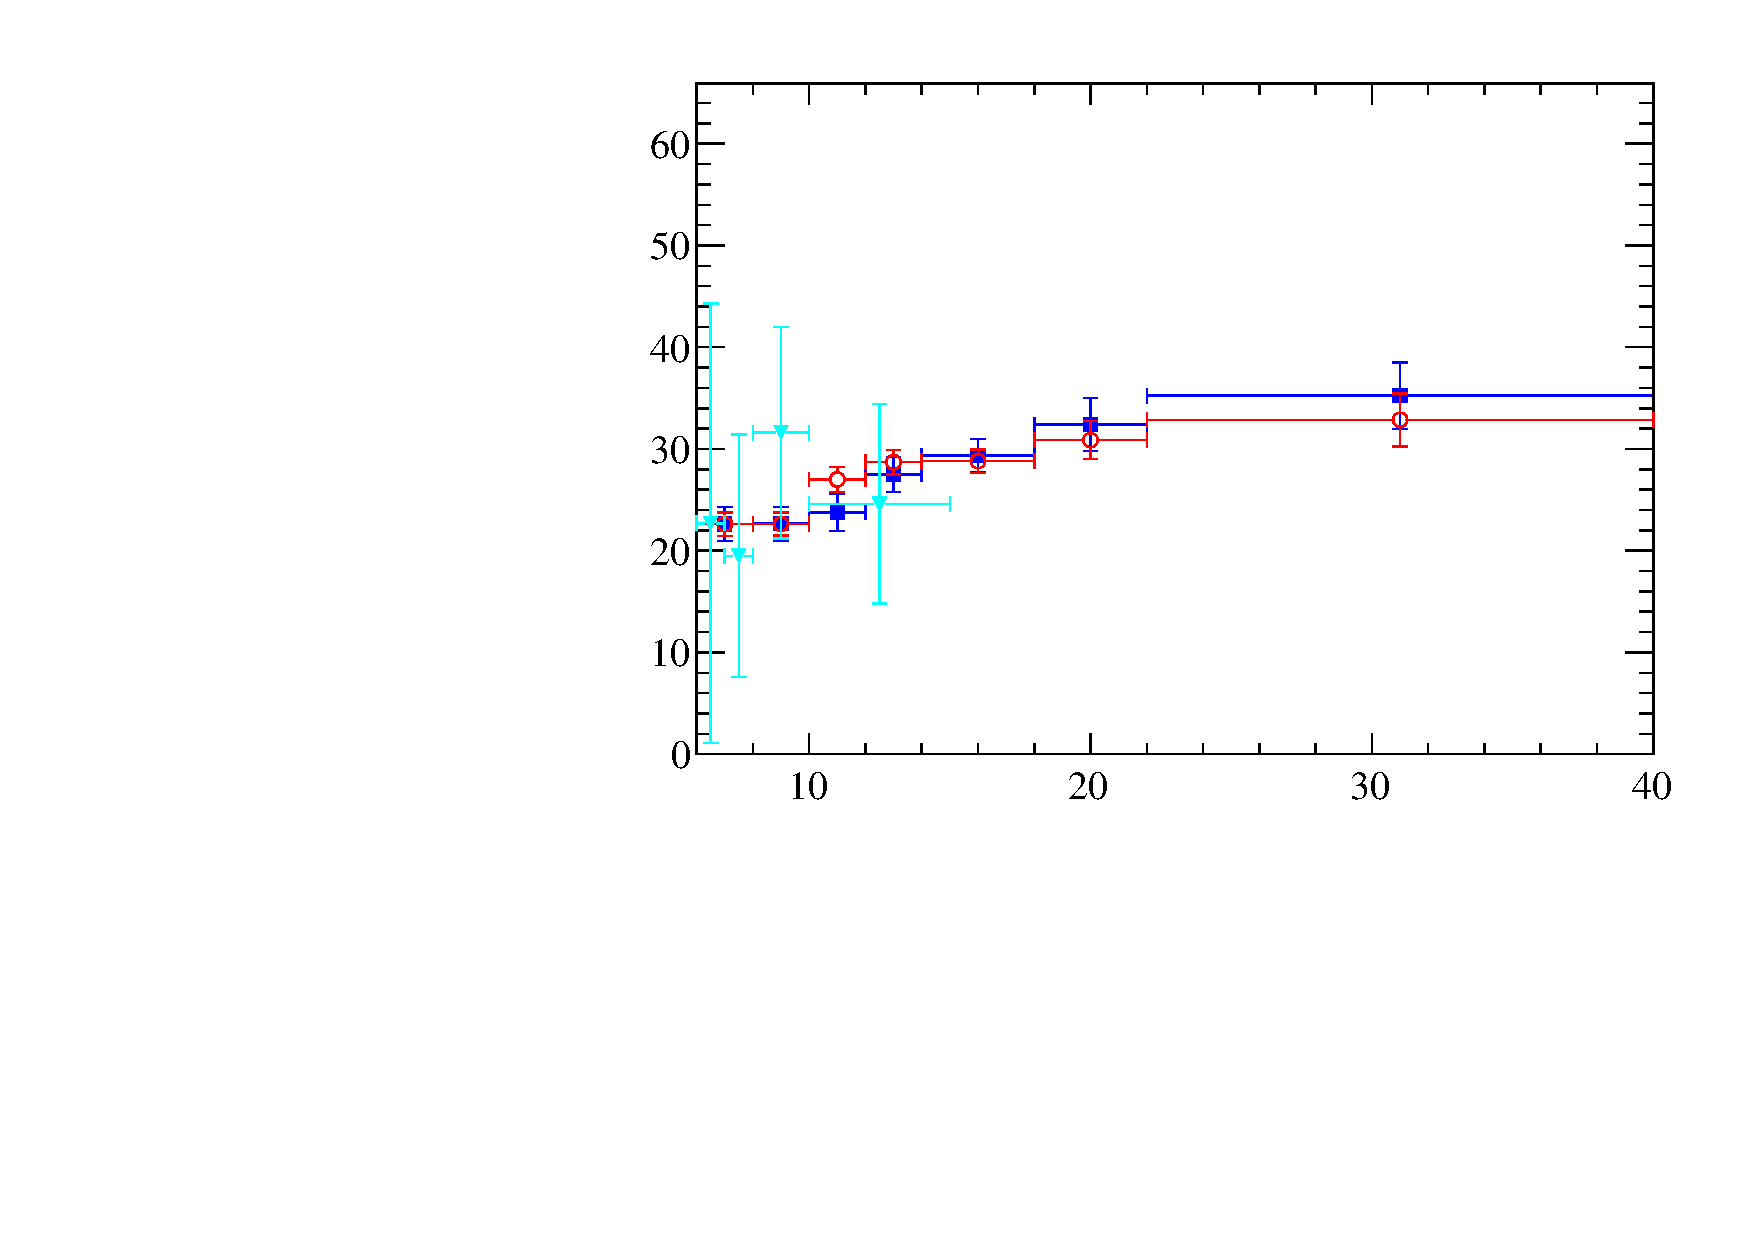
\includegraphics[width=75mm, height=60mm]{frac-1s/cb1p_ups1s_2010}
    }
    \put(2,145){\begin{sideways}\Y1S fraction, \% \end{sideways}}
    \put(35,122){$p_T^{\Y1S} \left[\gevc\right]$}

    \put(45,173){\scriptsize $\chibOneP \to \Y1S \gamma$}
    \put(48,168){\scriptsize \textcolor{blue}{\sqs=7\tev}}
    \put(48,164){\scriptsize \textcolor{red}{\sqs=8\tev}}
    \put(48,160){\scriptsize \textcolor{cyan}{\sqs=7\tev (2010)}}
    
    \put(43,168){
\includegraphics[width=3mm, height=2mm]{bsf}}
    \put(43,164){
\includegraphics[width=3mm, height=2mm]{rco}}
    \put(43,160){
\includegraphics[width=3mm, height=2mm]{ctuc}}
    %% =======================================================================
    \put(75,120){
      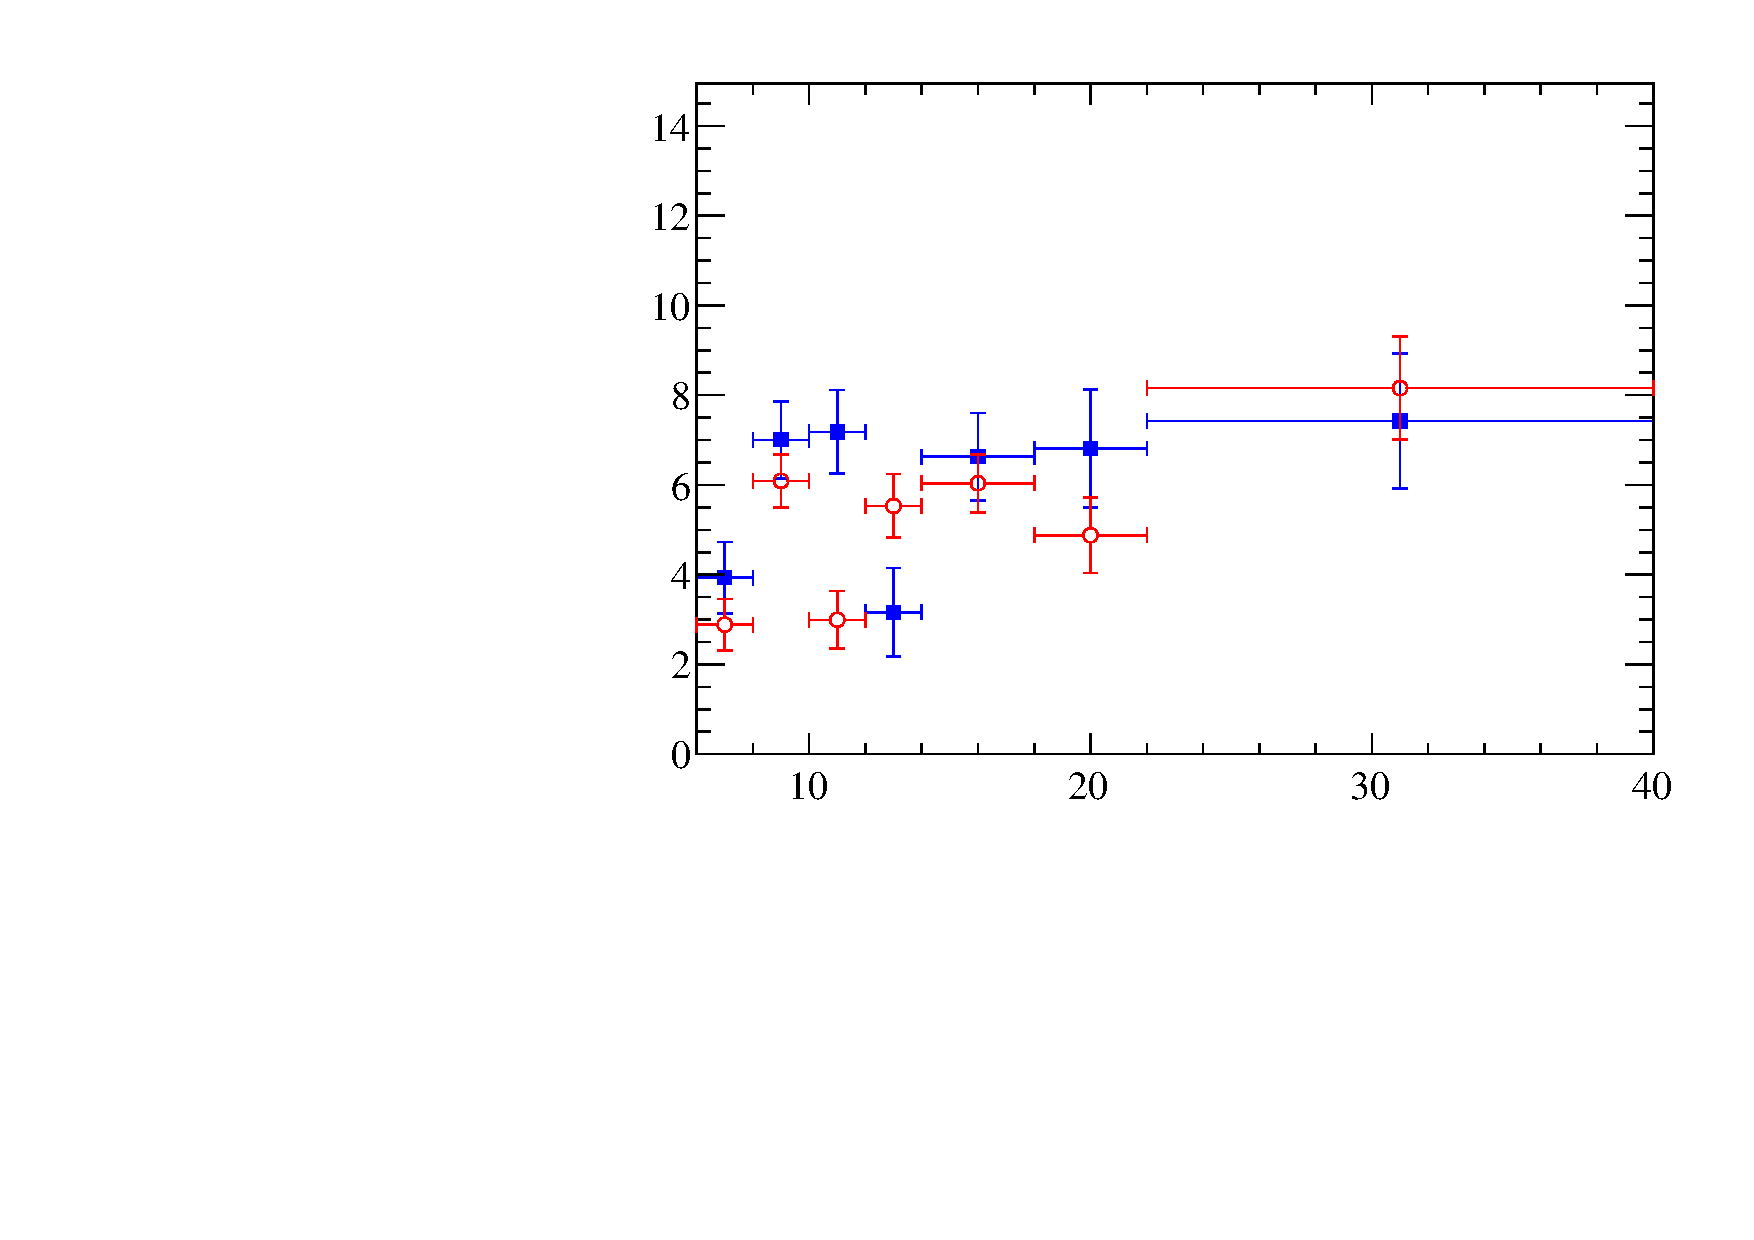
\includegraphics[width=75mm, height=60mm]{frac-1s/cb2p_ups1s}
    }
    \put(77,145){\begin{sideways}\Y1S fraction, \% \end{sideways}}
    \put(110,122){$p_T^{\Y1S} \left[\gevc\right]$}

    \put(120,173){\scriptsize $\chibTwoP \to \Y1S \gamma$}
    \put(123,168){\scriptsize \textcolor{blue}{\sqs=7\tev}}
    \put(123,164){\scriptsize \textcolor{red}{\sqs=8\tev}}
    
    
    \put(118,168){
\includegraphics[width=3mm, height=2mm]{bsf}}
    \put(118,164){
\includegraphics[width=3mm, height=2mm]{rco}}
    
    %% =======================================================================
    \put(0,60){
      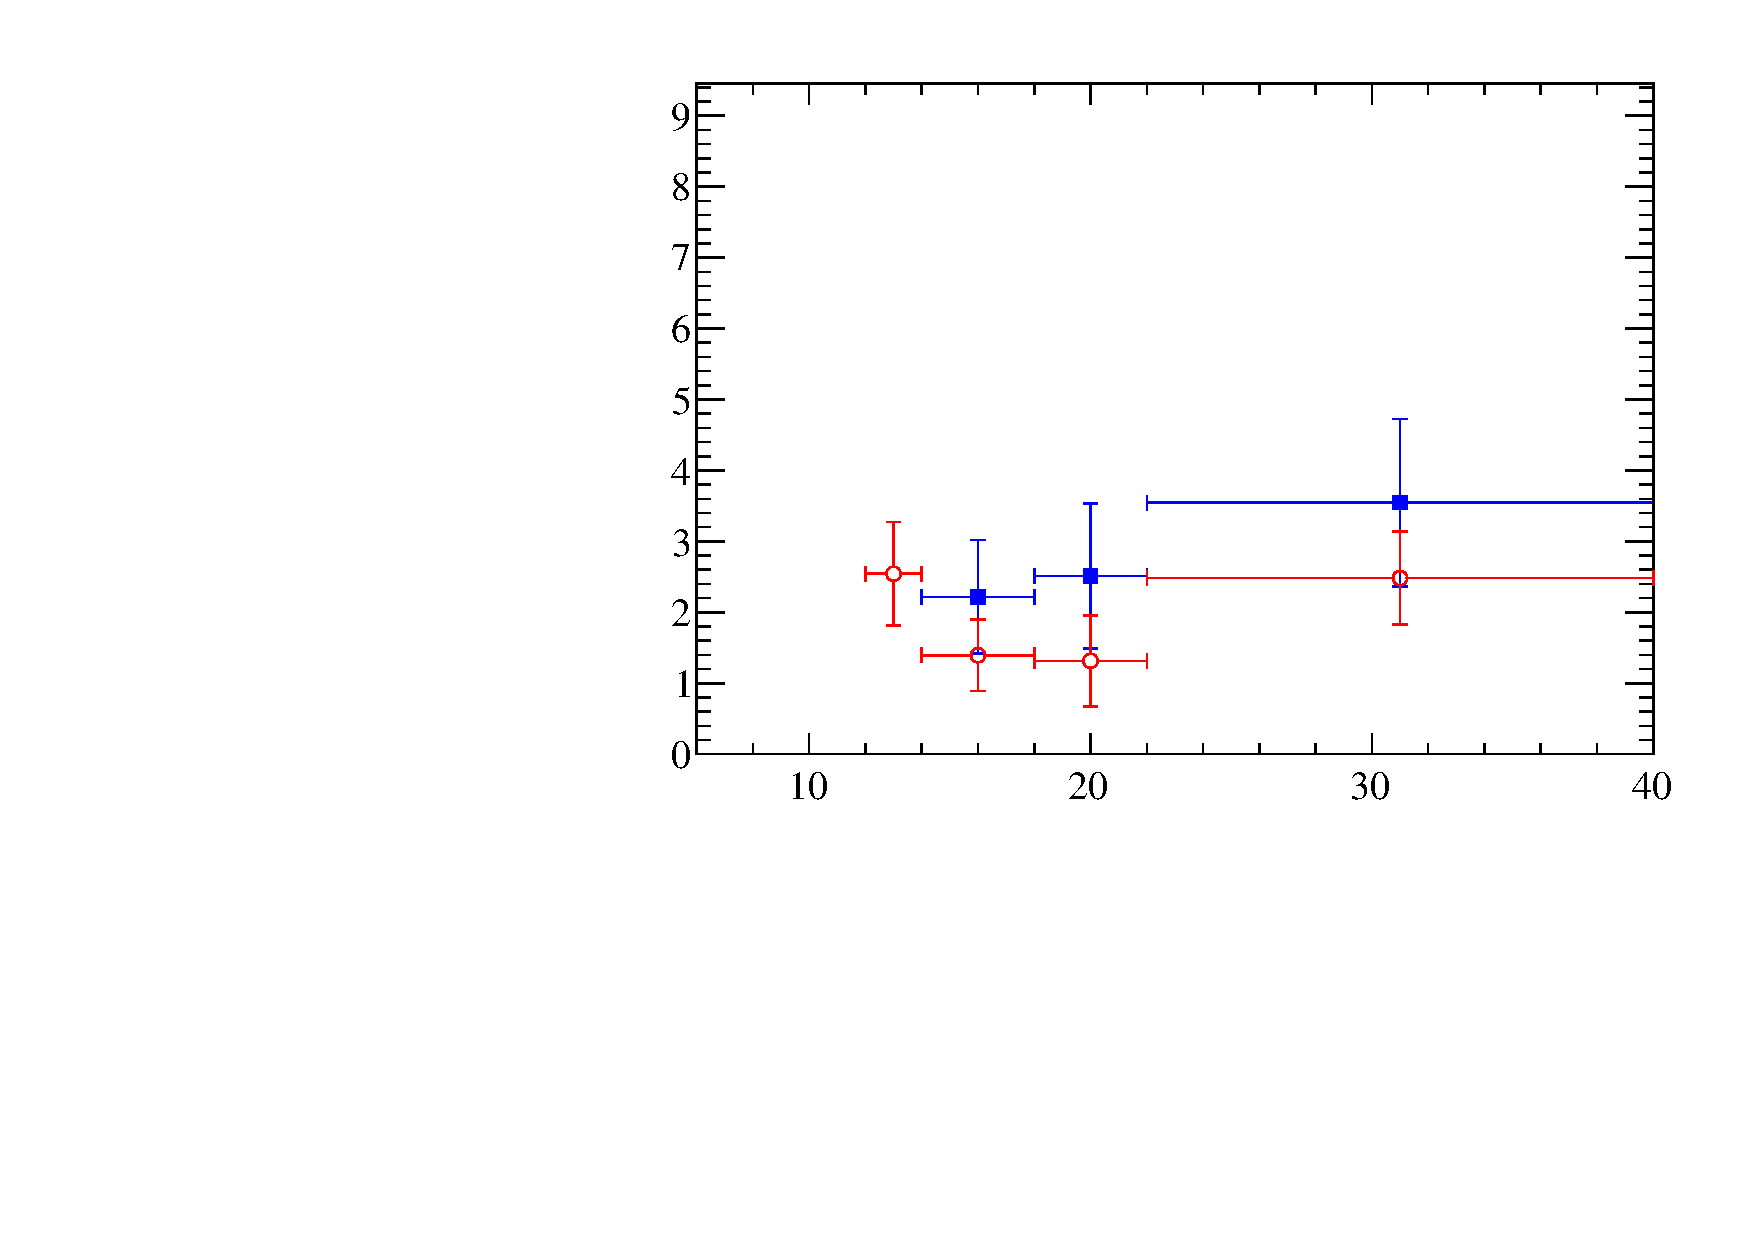
\includegraphics[width=75mm, height=60mm]{frac-1s/cb3p_ups1s}
    }
    \put(2,85){\begin{sideways}\Y1S fraction, \% \end{sideways}}
    \put(35,62){$p_T^{\Y1S} \left[\gevc\right]$}

    \put(45,113){\scriptsize $\chibThreeP \to \Y1S \gamma$}
    \put(48,108){\scriptsize \textcolor{blue}{\sqs=7\tev}}
    \put(48,104){\scriptsize \textcolor{red}{\sqs=8\tev}}
    
    
    \put(43,108){
\includegraphics[width=3mm, height=2mm]{bsf}}
    \put(43,104){
\includegraphics[width=3mm, height=2mm]{rco}}
    
    %% =======================================================================
    \put(75,60){
      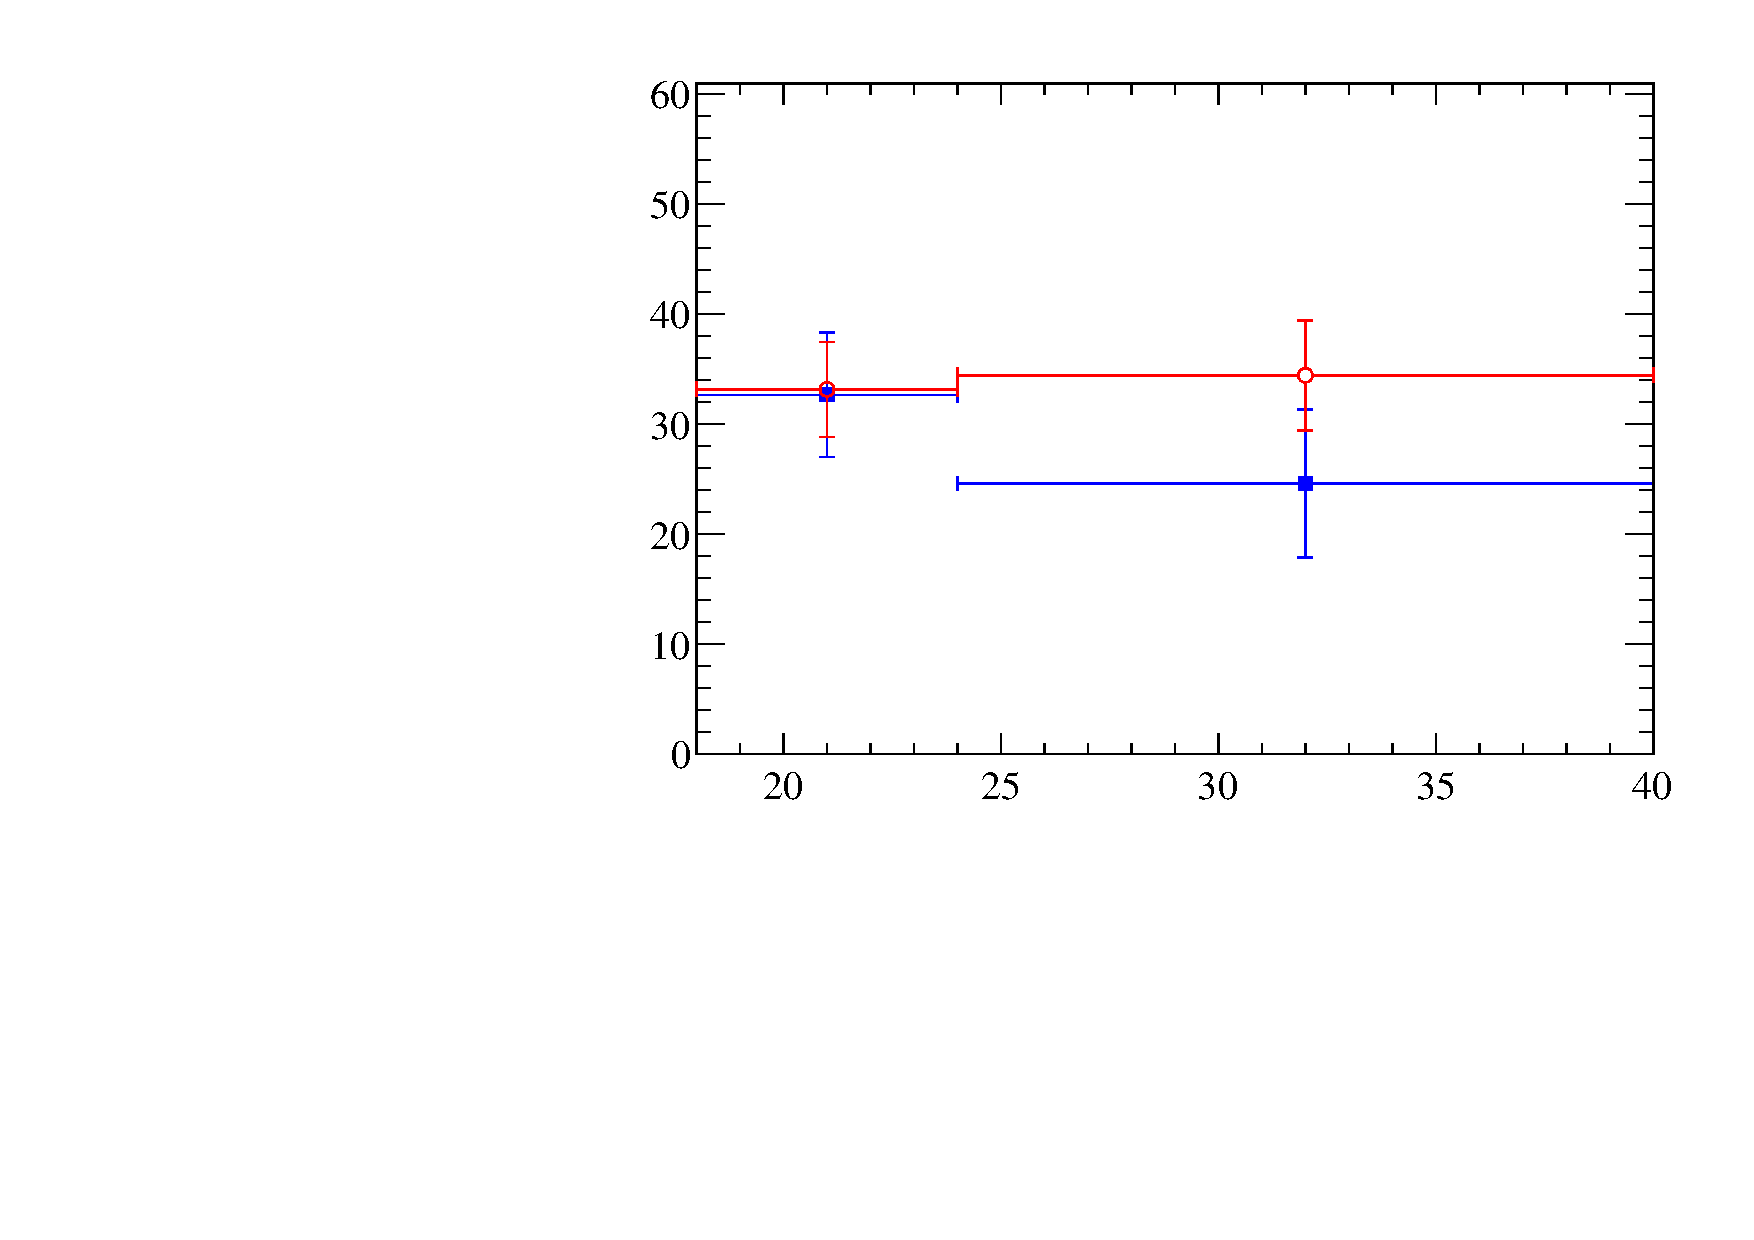
\includegraphics[width=75mm, height=60mm]{frac-1s/cb2p_ups2s}
    }
    \put(77,85){\begin{sideways}\Y2S fraction, \% \end{sideways}}
    \put(110,62){$p_T^{\Y2S} \left[\gevc\right]$}

    \put(120,113){\scriptsize $\chibTwoP \to \Y2S \gamma$}
    \put(123,108){\scriptsize \textcolor{blue}{\sqs=7\tev}}
    \put(123,104){\scriptsize \textcolor{red}{\sqs=8\tev}}
    
    
    \put(118,108){
\includegraphics[width=3mm, height=2mm]{bsf}}
    \put(118,104){
\includegraphics[width=3mm, height=2mm]{rco}}
    
    %% =======================================================================
    \put(0,0){
      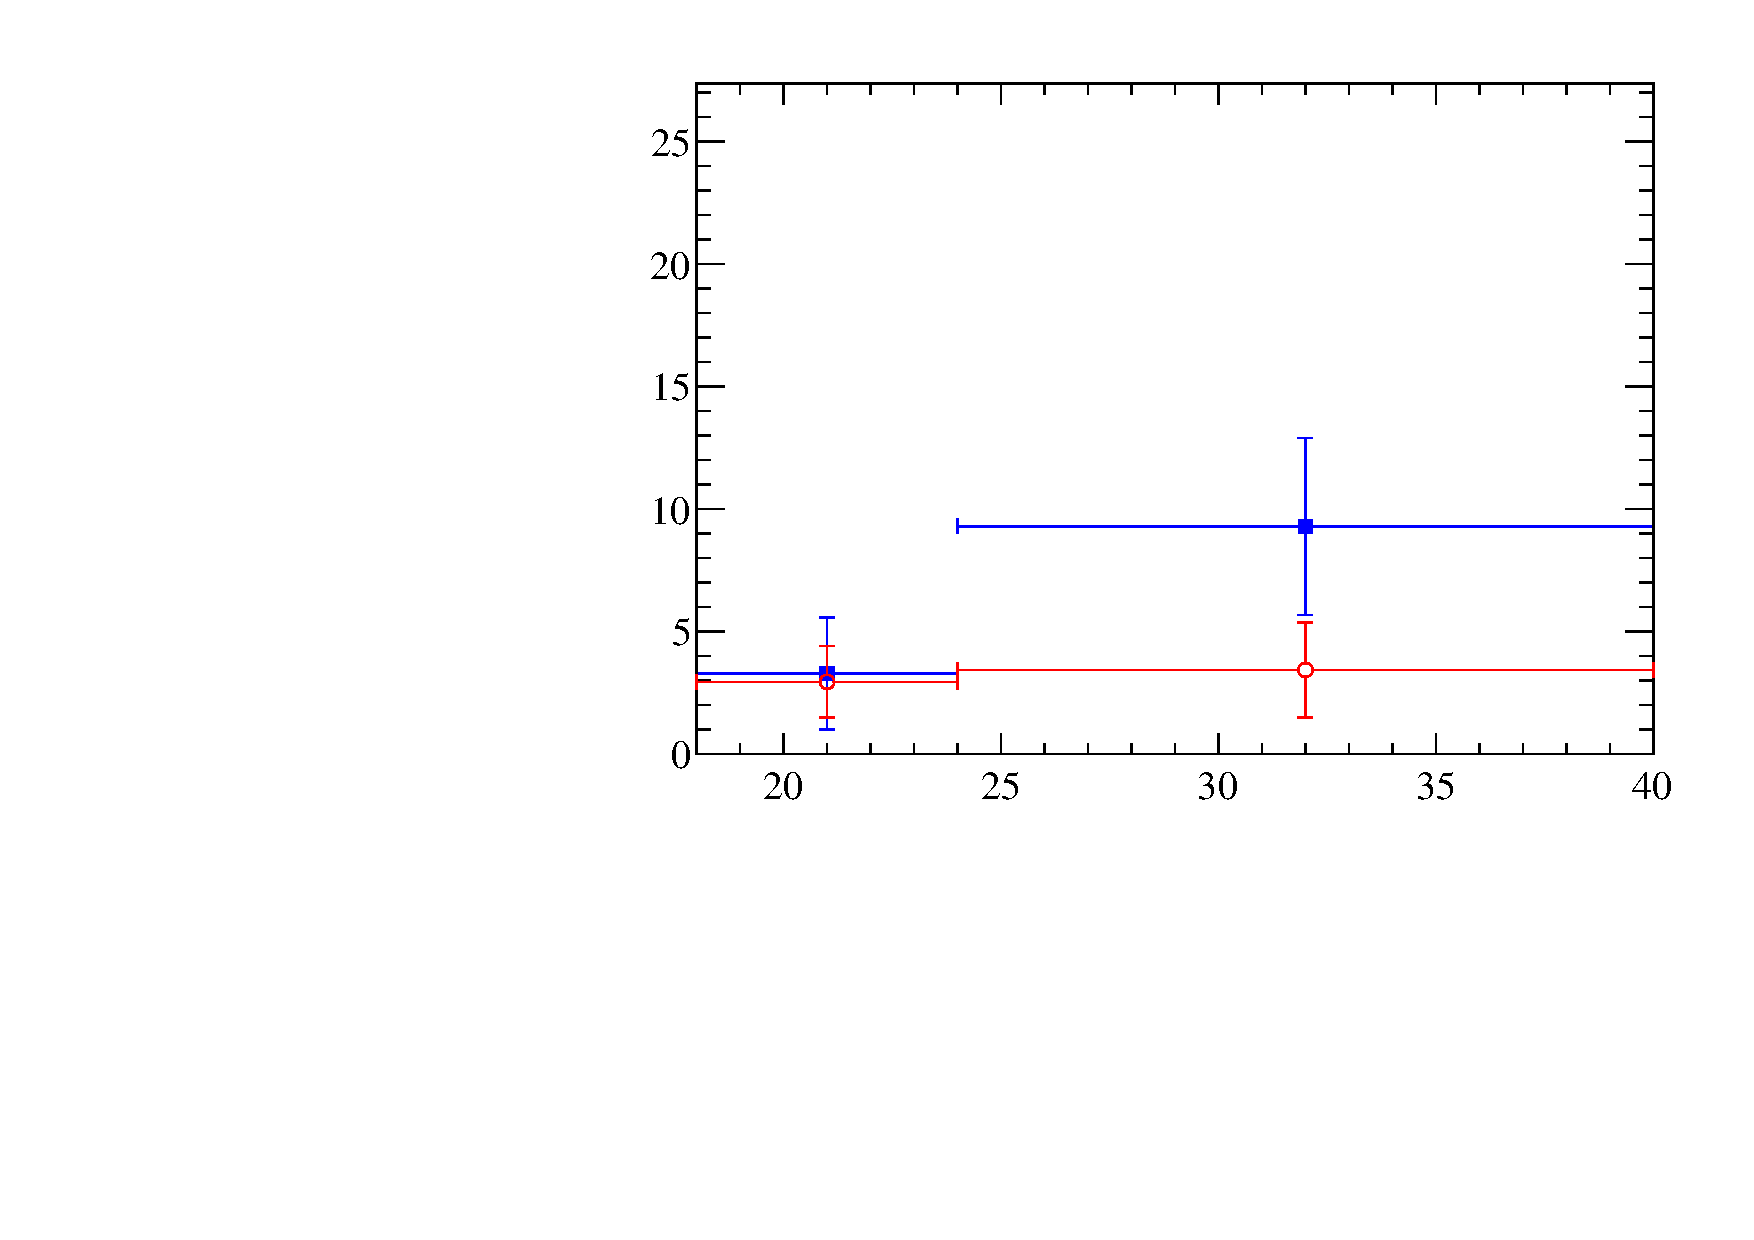
\includegraphics[width=75mm, height=60mm]{frac-1s/cb3p_ups2s}
    }
    \put(2,25){\begin{sideways}\Y2S fraction, \% \end{sideways}}
    \put(35,2){$p_T^{\Y2S} \left[\gevc\right]$}

    \put(45,53){\scriptsize $\chibThreeP \to \Y2S \gamma$}
    \put(48,48){\scriptsize \textcolor{blue}{\sqs=7\tev}}
    \put(48,44){\scriptsize \textcolor{red}{\sqs=8\tev}}
    
    
    \put(43,48){
\includegraphics[width=3mm, height=2mm]{bsf}}
    \put(43,44){
\includegraphics[width=3mm, height=2mm]{rco}}
    
  % \graphpaper[5](0,0)(75, 60)
  \end{picture}
 }

\column{.4\textwidth}
\begin{itemize}
\item For $\chi_b(1P)$ decay the fraction is consistent with the previous
results.
 \item About 40\% of $\Upsilon$ come from $\chib$, with a mild transverse
 momentum dependence.
\item $\chi_b(3P)$ fraction in $\Upsilon(3S)$ decay is $34 \pm 7$ \% for
$24<p_T^{\Upsilon(3S)}<40\gevc$.
\end{itemize}
\end{columns}


\end{frame}